\renewcommand\thesection{XIV}
\section{Circuits à Courant Alternatif: Impédance, Puissance, Facteur de Qualité, et Largeur de Bande}


\begin{multicols*}{2}
    \subsection{Impédance Complexe}
    Valeur généralisant la notion de résistance, réactance capacitive, et réactance inductive: elle caractérise la manière dont le circuit freine le courant.
    
    \[ Z = \frac{\tilde v}{\tilde i} \]
    
    \begin{center}
        \begin{tikzpicture}[scale=0.5]
            \draw[->] (0,0) -- (0, 4) node[above] {$\tilde v_L$};
            \draw[->] (0,0) -- (5, 0) node[above] {$\tilde v_R$};
            \draw[->] (0,0) -- (2.5, 0) node[below] {$\tilde i$};
            \draw[->] (0,0) -- (0, -2) node[below] {$\tilde v_C$};
            \draw[->] (0,0) -- (5, 2) node[above] {$\tilde v$};
            \draw[->] (3, 0) arc (0:33:2) node[right, pos=0.6] {$\varphi$};
        \end{tikzpicture}
    \end{center}
    
    
    \[ |Z| = \left| \frac{\tilde v}{\tilde i} \right| = \left| \frac{v_0 e^{j\varphi}}{i_0} \right| = \frac{v_0}{i_0} = \frac{v_{\text{eff}}}{i_{\text{eff}}} \]
    
    \paragraph{Relation entre Impédance et Déphasage}
    \[ \cos \varphi = \frac{\Re\{Z\}}{|Z|} \qquad et \qquad \tan \varphi = \frac{\Re\{Z\}}{\Im\{Z\}}\]
    
    \subsubsection{Résistances}
    
    \[ Z_R = \frac{v_{0R}}{I_0} = \frac{RI_0}{i_0} = R \]
    
    Car $\tilde i = i_0e^{j\varphi}$ et $\tilde v = v_{0R} e^{j\varphi}$ ont un déphasage nul.
    
    \[ \Rightarrow Z_R = |Z_R| = R \]
    
    \subsubsection{Condensateurs}
    
    \[ Z_C = \frac{-V_{0C} j}{i_0} = \frac{\frac{-i_0}{\omega C}}{i_0} j = \frac{-j}{\omega C} = \frac{1}{\omega C j} \]
    
    Comme $-j^2 = 1 \Leftrightarrow -j = \frac{1}{j}$.
    
    \begin{align*}
        Z_C &= -X_C j \\
        |Z_C| &= X_C
    \end{align*}
    
    
    \subsubsection{Inducteurs}
    
    \begin{align*}
        Z_L &= \frac{V_{0L}j}{i_0} = \frac{\omega L i_0}{i_0}j = \omega L j \\
        \Rightarrow Z_L &= X_L j \\
        |Z_L| &= X_L
    \end{align*}
    
    \subsection{Impédance d'un Circuit RLC en Série}
    
    \begin{align*}
        Z &= \frac{\tilde v}{\tilde i} = \frac{V_{0R} + (V_{0L} - V_{0C})j}{i_0} \\
         &= \frac{V_{0R}}{i_0} + \left( \frac{V_{0L}}{i_0} - \frac{V_{0C}}{i_0} \right) j \\
         \Rightarrow Z &= R + \left(\omega L - \frac{1}{\omega C}\right)j \\
         |Z| &= \sqrt{R^2 + \left(\omega L - \frac{1}{\omega C}\right)^2}
    \end{align*}
    
    \subsection{Impédences en série et en parallèle}
    
    \subsubsection{En série}
    
    \begin{center}
        \begin{circuitikz}
            \draw (0, 0) to [vsourcesin] (3, 0) to [generic = $Z_3$] (3,2) to [generic = $Z_2$] (0,2) to [generic = $Z_1$] (0,0);
        \end{circuitikz}
    \end{center}
    \[ Z_{\text{eq}} = \sum _{i = 1} ^n Z_i \]
    
    \subsubsection{En parallèle}
    
    \begin{center}
        \begin{circuitikz}
            \draw (0,0) to [vsourcesin] (0, 3);
            \draw (0, 3) to (2, 3) to [generic = $Z_1$] (2,0) to (0,0); 
            \draw (2, 3) to (3, 3) to [generic = $Z_2$] (3,0) to (2,0); 
            \draw (3, 3) to (4, 3) to [generic = $Z_3$] (4,0) to (3,0); 
        \end{circuitikz}
    \end{center}
    \[ \frac{1}{Z_{\text{eq}}} = \sum _{i = 1} ^n \frac{1}{Z_i} \]
    
    \subsection{Puissance Dissipée en AC}
    
    La puissance électrique instantanée en AC est donnée par:
    \[ p = vi \]
    
    \subsubsection{Résistances}
    
    \[ p = Ri^2 = Ri_0^2 \sin^2(\omega t) \]
    
    Avec un taux moyen de:
    \[ \langle p \rangle = i_{\text{eff}}^2 R = \frac{V^2_{\text{eff}}}{R} \]
    
    \subsubsection{Condensateurs}
    
    \[ p = v_{0C} \sin(\omega t - \frac{\pi}{2}) i_0 \sin(\omega t)) = -\frac{V_{0C}^2 C}{2} \sin(2 \omega t) \]
    
    \[ \langle p \rangle = -\frac{1}{T} \int_0^T \frac{V_{0C}^2 C}{2} \sin(2 \omega t) dt = 0 \]
    
    Un condensateur ne dissipe pas d'énergie sur un nombre demi-entier de périodes. Pendant un quart de cycle, le condensateur emmagasine de l'énergie: $vi$ est positif; pendant le quart suivant du cycle: $vi$ est négatif. Ce qui s'additionne pour donner une puissance nulle.
    
    Une résistance n'emmagasine pas l'énergie: elle la dissipe en chaleur et ne la restitue donc pas à la source.
    
    \begin{center}
        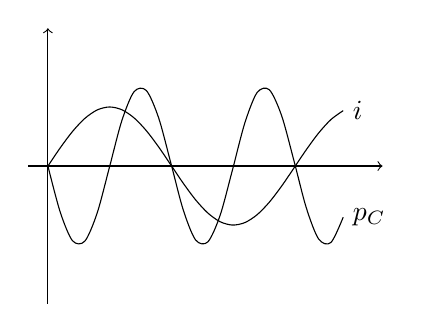
\begin{tikzpicture}[scale=0.5,domain=0:7.5,smooth]
            \draw[->] (0, -3.5) to (0, 3.5);
            \draw[->] (-0.5, 0) to (8.5, 0);
            \draw plot (\x, {1.5* sin(\x r)}) node[right] {$i$};
            \draw plot (\x, {-2 *sin((2 * \x) r)}) node[right] {$p_C$};
        \end{tikzpicture}
    \end{center}
    
    \subsubsection{Inducteurs}
    \[ p = v_{0L} \sin(\omega t + \frac{\pi}{2}) i_0 \sin(\omega t) = \frac{1}{2} v_{0L} i_0 \sin(2\omega t) \]
    
    \[ \langle p \rangle = \frac{1}{T} \int_0^T \frac{1}{2} \frac{V_{0L}^2}{\omega L}\sin(2\omega t) dt = 0 \]
    
    Pour les même raisons que pour un condensateur, la puissance moyenne d'un inducteur est nulle.
    
    \begin{center}
        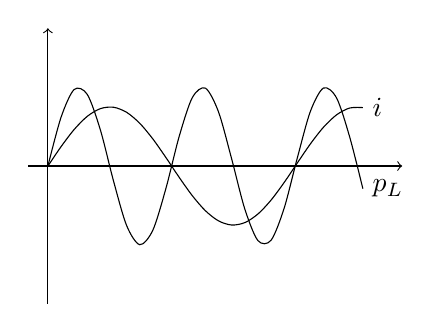
\begin{tikzpicture}[scale=0.5,domain=0:8,smooth]
            \draw[->] (0, -3.5) to (0, 3.5);
            \draw[->] (-0.5, 0) to (9, 0);
            \draw plot (\x, {1.5* sin(\x r)}) node[right] {$i$};
            \draw plot (\x, {2 *sin((2 * \x) r)}) node[right] {$p_L$};
        \end{tikzpicture}
    \end{center}
    
    \subsubsection{Puissance moyenne}
    
    Seule la partie résistive du circuit dissipe de l'énergie.
    
    \begin{align*}
        \langle p \rangle &= \Re \{Z\} i^2_{\text{eff}} \\
        \Rightarrow \langle p \rangle &= i_{\text{eff}}v_{\text{eff}} \cos\varphi
    \end{align*}
    
    \subsection{Phénomène de résonance}
    
    Alors que la composante réelle résistive d'une impédance ne dépend pas de la fréquence angulaire $\omega$, la partie imaginaire vaire avec celle-ci. D'où dans un circuit non purement résistif $|Z|$ varie avec $\omega$ et donc $I_{\text{eff}}$ varie avec $\omega$ pour $V_{\text{eff}}$ fixe.
    
    \paragraph{Fréquence de Résonnance}
    Fréquence angulaire $\omega_0$ telle que $|Z|$ atteint un minimum et donc $i$ atteint un maximum.
    
    \subsubsection{Fréquence de Résonnance pour un Circuit RLC}
    
    Pour un circuit RLC, $\omega_0$ et $i_{\text{eff}}^{\text{max}}$ valent:
    
    \[ \omega_0 = \frac{1}{\sqrt{LC}} \qquad \text{et} \qquad i_{\text{eff}}^{\text{max}} = \frac{V_{\text{eff}}}{R} \]
    
    \subsection{Facteur de Qualité}
    
    Défini comme:
    \[ Q = \frac{2\pi \cdot \text{énergie max emmagasinée dans le circuit}}{\text{énergie dissipée par cycle}} \]
    
    \subsubsection{Circuit RLC en Série} 
    À la résonnance, le facteur de qualité vaut:
    \[ Q_0 = \frac{1}{R} \sqrt{\frac{L}{C}} \]
    
    \subsection{Largeur de Bande}
    BW ou Bandwidth en anglais.
    
    Différence entre deux fréquences auquelles le courant ne vaut que $\frac{1}{\sqrt{2}}$ fois le courant maximum.
    
    \[ BW = f_2 - f_1 \]
    
    \begin{center}
        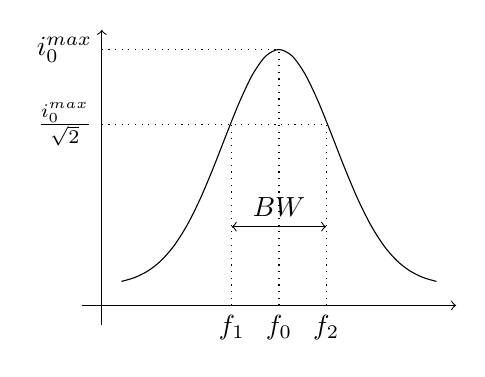
\begin{tikzpicture}[domain=0.25:4.25, scale=1, smooth]
            \draw[->] (0, -0.25) to (0, 3.5);
            \draw[->] (-0.25, 0) to (4.5, 0);
            \draw plot (\x, {3* exp(-(\x-2.25)^2) + 0.25});
            \draw[dotted] (0, {3* exp(0)^2 + 0.25}) node[left] {$i_0^{\text{max}}$} -- (2.25, {3* exp(0)^2 + 0.25});
            \draw[dotted] (0, {(3* exp(0)^2 + 0.25)/sqrt(2)}) node[left] {$\frac{i_0^{\text{max}}}{\sqrt{2}}$} -- (2.85, {(3* exp(0)^2 + 0.25)/sqrt(2)});
            \draw[dotted] (2.25, 0) node[below] {$f_0$} -- (2.25, {3* exp(0)^2 + 0.25});
            \draw[dotted] (1.65, 0) node[below] {$f_1$} -- (1.65, {(3* exp(0)^2 + 0.25)/sqrt(2)});
            \draw[dotted] (2.85, 0) node[below] {$f_2$} -- (2.85, {(3* exp(0)^2 + 0.25)/sqrt(2)});
            
            \draw[<->] (1.65, 1) -- (2.85, 1) node[pos=0.5, above] {$BW$};
        \end{tikzpicture}
    \end{center}
    
    \subsubsection{Circuit RLC en Série}
    
    Pour le circuit RLC en série, on établit la relation entre la largeur de bande et le facteur de qualité:
    \[ Q_0 = \frac{f_0}{DW} \]
    
\end{multicols*}